\documentclass{ctexbeamer}
\usetheme[navigation]{UMONS}
\usepackage[]{inputenc}
\usepackage[english]{babel}
\usepackage{tikz}
\usetikzlibrary{fadings}


\title[互联网求职经验分享]{互联网求职经验分享}
\author[彭宗宇]{彭宗宇}
\institute[DLUT]{%
	大连理工大学
}
\date{\today}

\AtBeginSection[]
{
	\begin{frame}<beamer>
		\frametitle{\textbf{目录}}
		\tableofcontents[currentsection]

	\end{frame}
}

\begin{document}
\maketitle

\begin{frame}
	\frametitle{\textbf{目录}}
	\tableofcontents
\end{frame}


\section{关于我}
\begin{frame}{关于我}
	\begin{enumerate}[<+-| alert@+>]
		\item 本科就读于中国地质大学(北京) 数学与应用数学
		      % \item 发表 sci 论文一篇
		\item 硕士就读于大连理工大学  应用数学
		\item 华为杯全国三等奖
		\item CSDN 博客专家
		\item 有一段实习: 百度语音技术部 C++ 开发
		\item 秋招收到 多乐游戏, 理想汽车, 百度语音技术部的 offer,  最后签 百度语音技术部
	\end{enumerate}

	\begin{block}{我的技术栈}<+->
		C/C++ 、 Python 、 Linux 、 Docker 、 Vim 、 Go 、 Lua 、 ......
	\end{block}
	% 一开始学习 Python , 但是 Python 岗位较少且没有竞争力, 就决定学一门静态语言. 
\end{frame}

% \begin{frame}
% 	\frametitle{}

% \end{frame}


\section{怎样准备}


\subsection{方向}
\begin{frame}{选好方向}
	明确自己想要什么, 确定了就坚持下去.
	\begin{enumerate}
		\item 感兴趣?
		\item 钱多?
		\item 事少?
		\item 离家近?
	\end{enumerate}

	数学专业可以选的方向很多... 国企/银行/教师/公务员/IT...

	\begin{exampleblock}{建议}
		做 IT 要有耐心, 要做好一直学习的打算,
		可能没有太多自己的时间.

		做自己喜欢的事情更重要.

		编程零基础可以试试测试开发/数据分析, 对代码要求不高.
	\end{exampleblock}
\end{frame}

\begin{frame}
	\frametitle{语言的选择}

	非科班要学很多基础课, 很多知识都是从零开始: 算法题要做, 基础八股要背, 底层(实现细节/原理)要了解, 项目也要懂...

	C++其实不适合后端求职, 除非深入学习细分方向:
	\begin{enumerate}
		\item 音视频/流媒体
		\item 操作系统/底层软件
		\item 游戏开发(适合喜欢玩游戏的同学)
		\item 量化交易(门槛高, 学历很重要)
		\item 嵌入式(稳定, 目前岗位需求大)
		\item AI 算法工程化
		\item 并行计算
		\item 数据库内核开发
		\item ...
	\end{enumerate}
\end{frame}
\begin{frame}
	\frametitle{语言的选择}
	Java 是互联网后端常用的, 目前推荐学 Java, 比较容易上手, 但是竞争更加激烈.

	Go 的岗位不多, 主要是字节跳动以及一些中厂在招人.

	\begin{exampleblock}{其他适合非科班的互联网赛道}
		\begin{enumerate}
			\item 测试开发(测试都是一套东西, 上手比较快)
			\item 数据分析(需要会 Python, 数据库等, 适合数学专业)
			\item 大数据开发(本质还是 Java的一些组件, 比较卷, 而且岗位少)
			\item 产品/市场(非技术类, 比较看重社交能力)
		\end{enumerate}
	\end{exampleblock}
\end{frame}

\begin{frame}
	\frametitle{题外话:  编辑器的选择}
	好的编辑器很重要, 初学者推荐 VS Code或者 jetbrains 系列 IDE. 
	逐渐熟悉之后可以使用 Vim. 
	刷力扣时候不要用 IDE, 实际笔/面试时候可能没有智能提示. 
	\begin{figure}\centering
		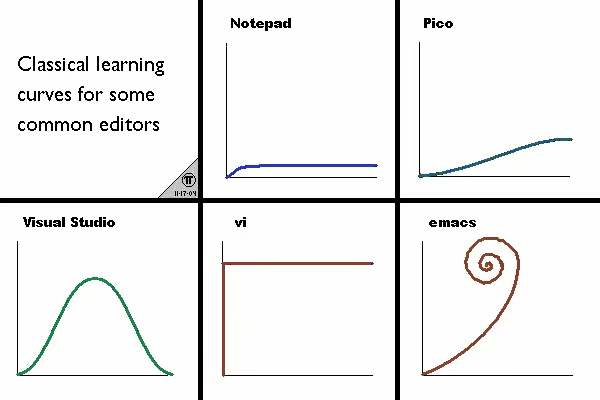
\includegraphics[width=.7\textwidth]{figures/editor.jpg}
	\end{figure}
\end{frame}

\subsection{求职前的准备}
\begin{frame}
	如果你真的热爱编程, 或者想多挣点钱: 
	\begin{alertblock}{学一项技术/语言/知识}
		知识密度: 看原始文档 > 看经典书籍 > 看视频

		时间成本: 看原始文档 < 看经典书籍 < 看视频
	\end{alertblock}
	重在总结和积累, 光看是不行的, 要上手自己写, 自己编译运行, 有好奇心.
	我看的一些书: (中英文对照看)
	\begin{enumerate}
		\item 语言学习: C++Primer, Effective C++, More Effective C++, Effective STL, ...
		\item 计算机基础: 深入理解计算机系统, 操作系统导论, Linux 系统编程手册, 网络是怎样连接的, ...
		\item 其它工具: Vim实用技巧,
	\end{enumerate}
	有的书要反复看, 有的书适合浏览略读.

	推荐用\textbf{微信读书}存电子书.
\end{frame}


\begin{frame}{一些有用的网站/工具}
	\begin{itemize}
		\item 刷算法题(准备笔试和面试): 力扣 (\hyperref[https://leetcode.cn]{leetcode.cn})
		\item 刷面试题/面经(准备面试, 求职交流): 牛客 (\hyperref[https://nowcoder.com]{nowcoder.com})
		\item 笔试真题解析: 公众号 万诺 coding / 塔子哥学算法
		\item 刷企业真题
		      \begin{itemize}
			      \item 赛码网(\hyperref[https://acmcoder.com]{acmcoder.com})
			      \item 牛客网(\hyperref[https://nowcoder.com]{nowcoder.com})
		      \end{itemize}
		\item 面试知识点: 小林 coding(\hyperref[https://xiaolincoding.com]{xiaolincoding.com})
		\item ChatGPT 是你的好帮手, 但是不能全盘相信(有一些知识点会一本正经地胡说八道), 要有自己的判断. 
	\end{itemize}
\end{frame}



\begin{frame}{求职过程中}
	不要焦虑, 坚持自己的目标, 按部就班去做. 
	多跟人交流, 分享信息, 多加几个群.
	\begin{itemize}
		\item 大工就业公众号(国企/研究所偏多)
		\item 各公司的招聘公众号, 最新的求职信息
		\item 海投网公众号
		\item 校招信息网
	\end{itemize}
\end{frame}

\begin{frame}{拿到 offer 之后}
	\begin{itemize}
		\item 比较薪资: offershow 小程序
		\item 加群交流
		\item 牛客发帖讨论
	\end{itemize}
\end{frame}

\section{有什么想了解的}

\begin{frame}
	\frametitle{有什么想了解的}

	我的微信: zorchp
\end{frame}

\begin{frame}{}
	\begin{center}
		\begin{tikzpicture}
			\node[above,xscale=1.5,yscale=1.4]{\Huge 谢谢!};
			% \node[xscale=1.2,above,yscale=-1.4,scope fading=south,opacity=0.5]{\huge Thank you!};
		\end{tikzpicture}
	\end{center}
\end{frame}

\end{document}
